% v2-acmtog-sample.tex, dated March 7 2012
% This is a sample file for ACM Transactions on Graphics
%
% Compilation using 'acmtog.cls' - version 1.2 (March 2012), Aptara Inc.
% (c) 2010 Association for Computing Machinery (ACM)
%
% Questions/Suggestions/Feedback should be addressed to => "acmtexsupport@aptaracorp.com".
% Users can also go through the FAQs available on the journal's submission webpage.
%
% Steps to compile: latex, bibtex, latex latex
%
% For tracking purposes => this is v1.2 - March 2012
\documentclass{sig-alternate} % V1.2

%\acmVolume{VV}
%\acmNumber{N}
%\acmYear{YYYY}
%\acmMonth{Month}
%\acmArticleNum{XXX}
%\acmdoi{10.1145/XXXXXXX.YYYYYYY}
\usepackage{graphicx}
%\usepackage[T2A]{fontenc} 
%\usepackage[utf8]{inputenc}
\usepackage{graphicx}
%\usepackage{indentfirst}
\usepackage{hyperref}
\usepackage{textcomp}

\begin{document}

\makeatletter
\def\@copyrightspace{\relax}
\makeatother

\title{Generalized LL parsing for context-free constrained path search problem}

\sloppy

\author{Semyon Grigorev\\
rsdpisuy@gmail.com\\
Saint Petersburg State University, Russia}

\maketitle

Path querying is an actual problem in bioinformatic, graph databases, ... One of specific problem is formal languages path problem~\cite{DirOfBigGraphAnalysis} which meens that paths constraints formulated as 
Query may be specified as context-free grammar: path $P = e_0,\dots,e_n$, $\omega = e_0.tag \cdot \dots \cdot e_n.tag$, $\omega \in L(G)$ 

Let we want to find all path with form $A^n B^n$. This constraint can not be specified with regular language as far as $L=\{a^n b^n; n>0\}$ is not regular but context free.
Required language can be specified by grammar $G$ presrnted in picture~\ref{grammarG}.

\begin{figure}[h]
   \begin{center}
\begin{verbatim}
s: A l | middle
middle: A B
l: s B
\end{verbatim}
   \caption{Grammar $G$ for language $L=\{a^n b^n; n>0\}$}
   \label{grammarG}        
   \end{center}
\end{figure}

We propose a context-free language constrained path problem solution which allow to find all paths and construct implicit representation of result. 

Our is based on generalized LL (GLL)~\cite{GLL} parsing algorithm which allow to process arbitrary context-free grammars.
Complexity is $O(n^3)$ in worst case and linear for unumbigues grammars, that better then complexity of CYK and Erly which used as base in other solutions.

All-path semantic --- SPPF constructed by algorithm contains all paths matched with specified constraints. SPPF for grammar $G$ and graph $M$ which presented in picture !!! is presented in picture !!!. 
Extensions allow to check whether path from $u$ to $v$ exists and extract it. For example ....

\begin{figure}[h]
    \begin{center}
        \includegraphics[width=6cm]{dot/input.pdf}
        \caption{xxx}
        \label{pic1}        
    \end{center}
\end{figure}

\begin{figure}[h]
    \begin{center}
        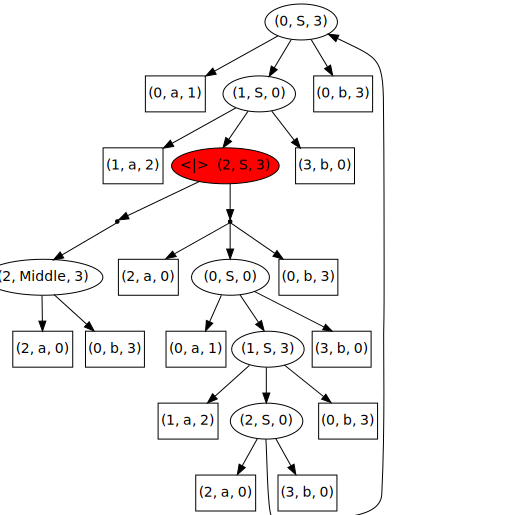
\includegraphics[width=9cm]{dot/AnBn.pdf}
        \caption{ccc}
        \label{pic1}        
    \end{center}
\end{figure}



Full index --- for dynamic graphs. It is necessary only recalculate ... This operation is native for basic algorithm.



%\begin{figure}
%    \begin{center}
%        \includegraphics[width=11cm]{input.pdf}
%        \caption{Входной граф}
%        \label{pic1}        
%    \end{center}
%\end{figure}
%


\begin{thebibliography}{9}
  
\bibitem{DirOfBigGraphAnalysis}
Miller, J. A., Ramaswamy, L., Kochut, K. J., \& Fard, A. (2015, June). Research Directions for Big Data Graph Analytics. In 2015 IEEE International Congress on Big Data (pp. 785--794). IEEE.

\bibitem{GLL}
Scott, E., \& Johnstone, A. (2010). GLL parsing. Electronic Notes in Theoretical Computer Science, 253(7), 177--189.

\bibitem{ConjCFPathQuery}
Hellings, J. (2014). Conjunctive context-free path queries.

\bibitem{PathQuerySemantic}
Hellings, J. (2015). Querying for Paths in Graphs using Context-Free Path Queries. arXiv preprint 
arXiv:1502.02242.

%\bibitem{CFPathQuery}
%Sevon, P., /& Eronen, L. (2008). Subgraph queries by context-free grammars. Journal of Integrative 
%Bioinformatics, 5(2), 100.

\end{thebibliography}

\end{document}
